%!TEX root = ../thesis.tex
\define{\chapterpath}{appendix}
\define{\imgpath}{appendix/img}

%%
\chapter{Appendix}
\label{appendix}

%%%%%%%%%%%%%%%%%%%%%%%%%%%%%%%%%%%%%%%%%%%%%%
%%%%%%%%%%%%%%%%%%%%%%%%%%%%%%%%%%%%%%%%%%%%%%
%%%%%%%%%%%%%%%%%%%%%%%%%%%%%%%%%%%%%%%%%%%%%%
%%%%%%%%%%%%%%%%%%%%%%%%%%%%%%%%%%%%%%%%%%%%%%
%%%%%%%%%%%%%%%%%%%%%%%%%%%%%%%%%%%%%%%%%%%%%%
\section{Illustration of the pick and place scenario}
\label{appendix:pickplace}

We illustrate in Figure~\ref{fig:lfui:pickplaceworld} the pick and place world of chapter~\ref{chpater:lfui} (where we used balls instead of cubes). There is three object that can be move in 4 different positions and stacked on two level maximum. The robot's gripper can move step by step at any of those four positions, grasp the object on top of the stack and release the object on top of a stack only if the stack is not full.

\begin{figure}[!ht]
  \centering
  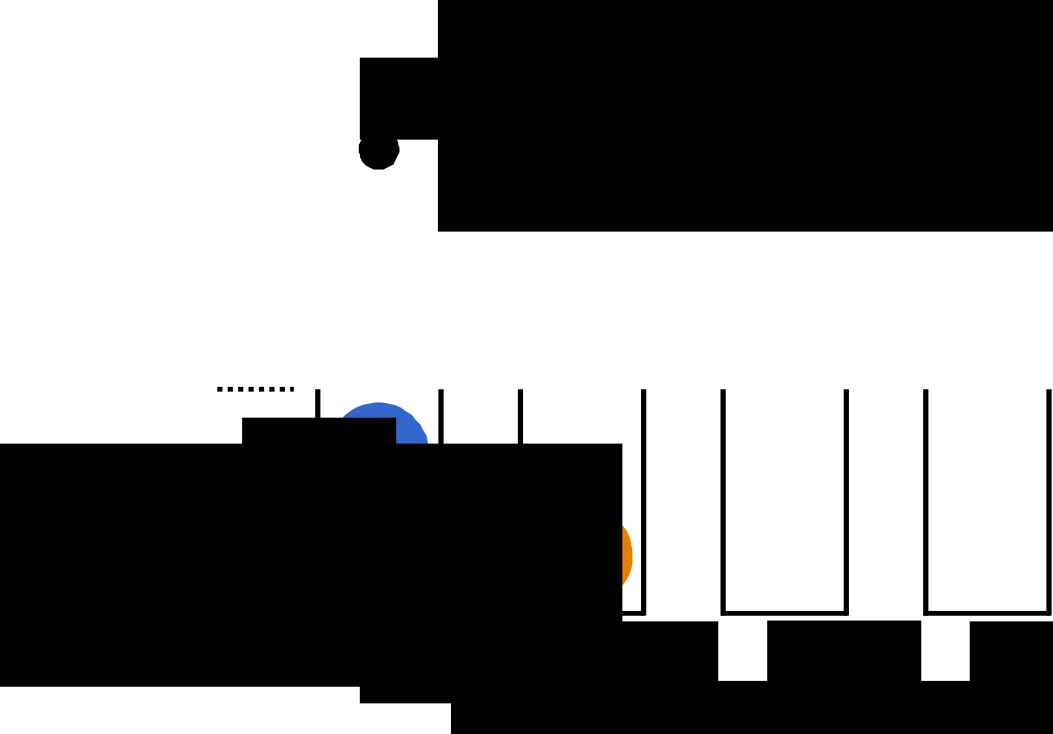
\includegraphics[width=\tworldsize\columnwidth]{\visualspdf/pick_and_place/pick_and_place_world.pdf}
  \caption{A schematic view of the pick and place problem. There is three object that can be move in 4 different positions and stacked on two level maximum. The robot's gripper can move step by step at any of those four positions, grasp the object on top of the stack and release the object on top of a stack only if the stack is not full.}
  \label{fig:lfui:pickplaceworld}
\end{figure}

In order to complete a task, i.e. to reach a specific configuration of ball, the robot as to perform an ordered sequence of action in order to move the ball in the appropriate way. In this example, we will consider only 3 out of the 624 possible hypothesis for illustration purpose. Figure~\ref{fig:lfui:pickplacesequence} shows a sequence of action starting in our hypothesis one configuration and going to our hypothesis 3 configuration in the shortest number of action as possible. Hypothesis 2 is a state on this path. While hypothesis 1 and hypothesis 3 seems ``close'' in terms of object position, they are actually far ``away'' one from an other in terms of action.

\begin{figure}[!ht]
  \centering
  \includegraphics[width=\columnwidth]{\visualspdf/pick_and_place/pick_and_place_sequence.pdf}
  \caption{A pick and place sequence showing the three hypothesis we will compare on our visuals examples and the sequence of actions from hypothesis 1 to hypothesis 3 through hypothesis 2. While hypothesis 1 and hypothesis 3 seems ``close'' in terms of object position, they are actually far ``away'' one from an other in terms of action.}
  \label{fig:lfui:pickplacesequence}
\end{figure}

For the case when the user is delivering feedback to the robot, the labeling process is presented in Figure~\ref{fig:lfui:pickplacefeedback} for a robot action randomly in the environment. Note that hypothesis 1 and 2 are the more difficult to discriminate by acting randomly as they share most of their optimal policies.

\begin{figure}[!ht]
  \centering
  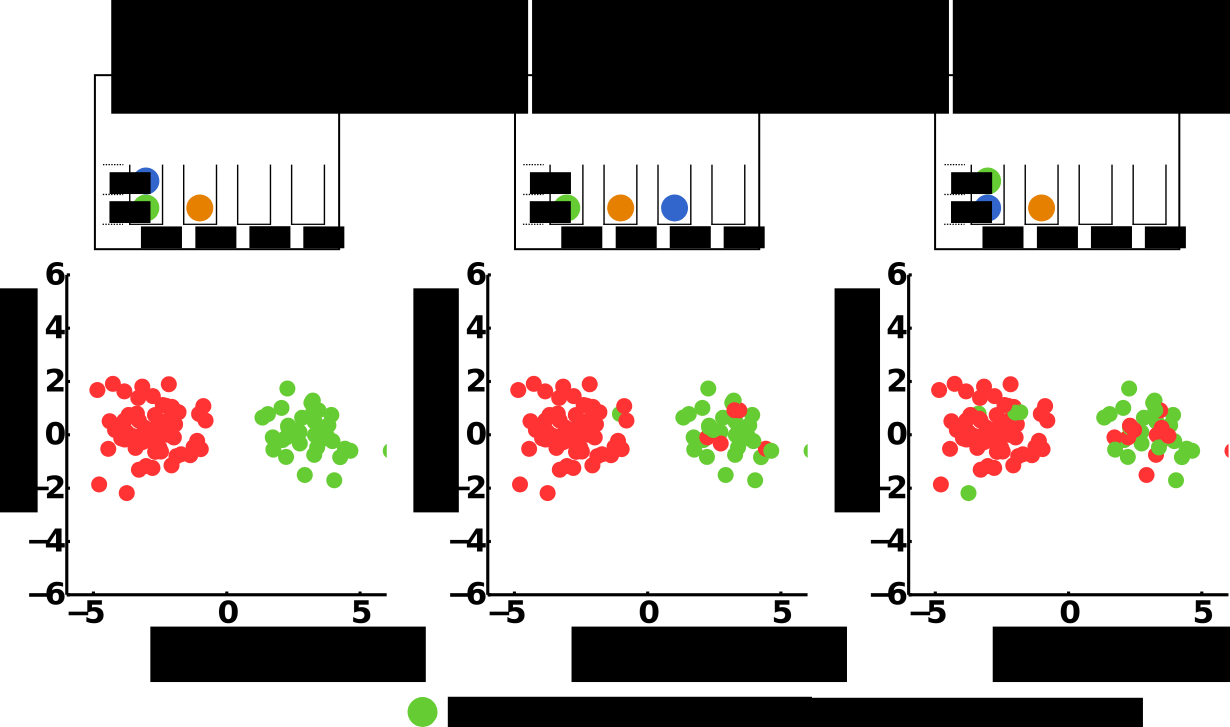
\includegraphics[width=\columnwidth]{\visualspdf/pick_and_place/pick_and_place_feedback.pdf}
  \caption{Results of the labeling process for our three hypothesis considering the feedback frame. The robot is exploring randomly the state space. The teacher is providing feedback with respect to hypothesis 1. Only a few state-action pairs allowed to differentiate between hypothesis 1 and 2.}
  \label{fig:lfui:pickplacefeedback}
\end{figure}


For the guidance case, the user uses the signals presented in Figure~\ref{fig:lfui:pickplaceguidancesignals} an the labeling process is presented in Figure~\ref{fig:lfui:pickplaceguidance} for a robot action randomly in the environment. Note that in some state there may be two optimal action to perform. For example, in Figure~\ref{fig:lfui:pickplacesequence}, for inverting two stacked balls there is two different optimal policies, either the one presented, or putting the blue ball in position 2 and the green in position 3 during the exchange of position. Those case make the learning process more difficult but we can still visually find out that only for hypothesis 1 that all points in one cluster share one color. This can be capture by our algorithm.

\begin{figure}[!ht]
  \centering
  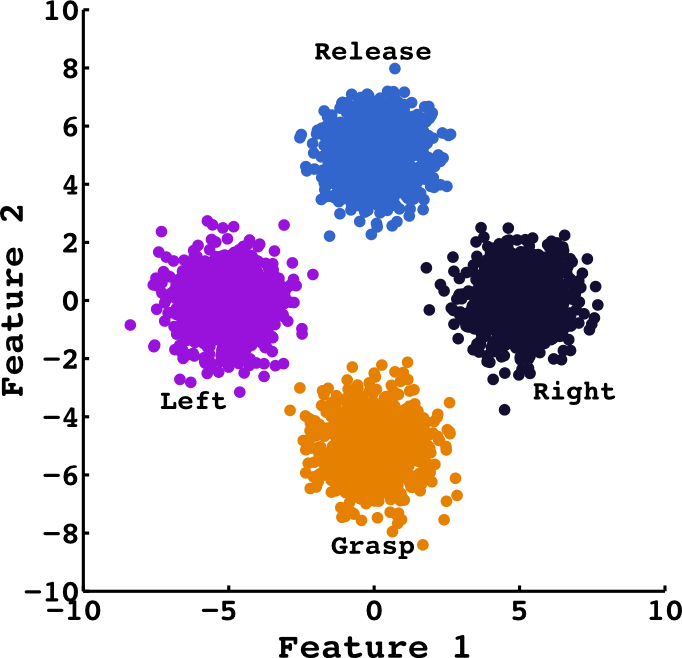
\includegraphics[width=\signalwidth\columnwidth]{\visualspdf/pick_and_place/guidance_pick_and_place.pdf}
  \caption{The guidance signals used by our simulated teacher for our visual examples.}
  \label{fig:lfui:pickplaceguidancesignals}
\end{figure}

\begin{figure}[!ht]
  \centering
  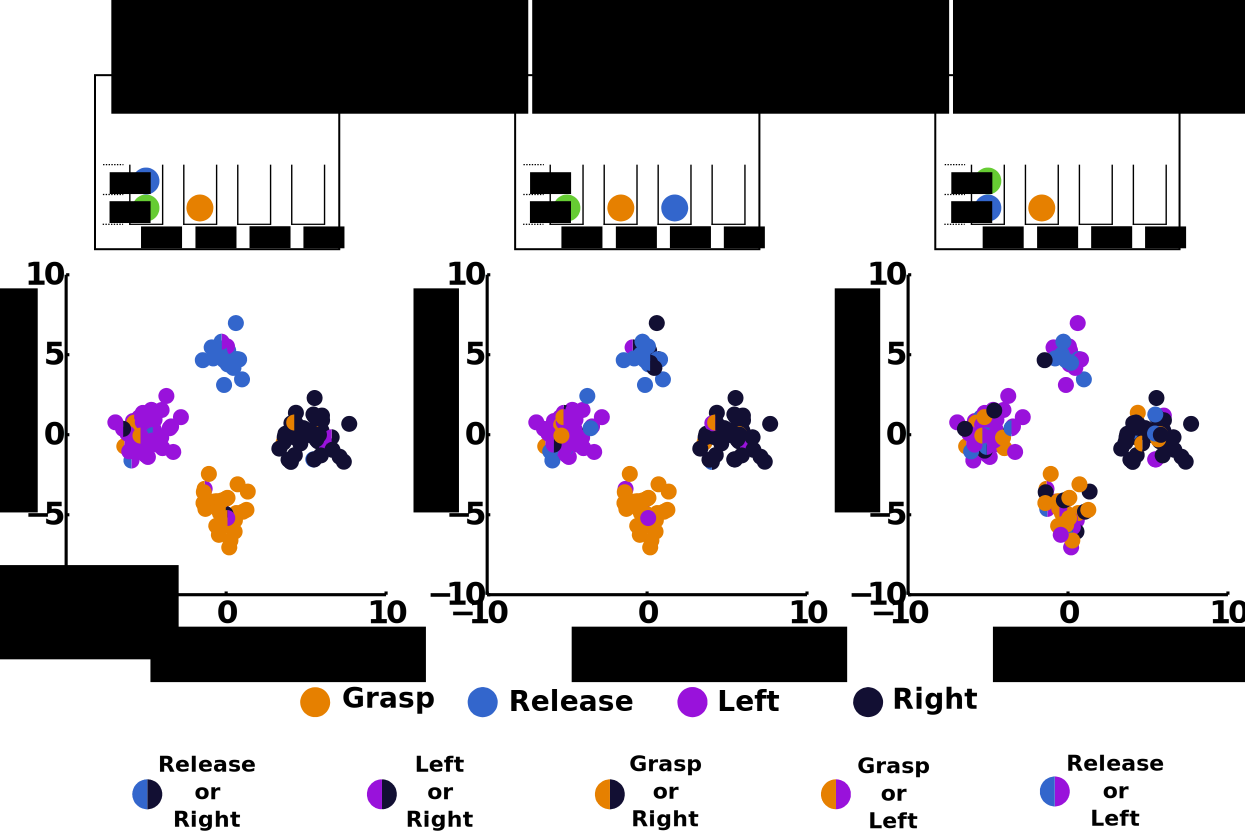
\includegraphics[width=\columnwidth]{\visualspdf/pick_and_place/pick_and_place_guidance.pdf}
  \caption{Results of the labeling process for our three hypothesis considering the guidance frame. The robot is exploring randomly the state space. The teacher is providing guidance with respect to hypothesis 1. The dot that contain two color are case where the user could have given two different guidance signals. It is only for hypothesis 1 that all points in one cluster share one color. The case of guidance with multiple optimal action in some state make the learning process more ambiguous and may require some additional time compared to the feedback case.}
  \label{fig:lfui:pickplaceguidance}
\end{figure}

We have provided an example of the pick and place world with two dimensional signals and considering only three hypothesis. In chapter~\ref{chapter:lfui:results}, we consider real spoken words mapped to a 20 dimensional space and the full space of hypothesis which consist of 624 possible object configurations.

%%%%%%%%%%%%%%%%%%%%%%%%%%%%%%%%%%%%%%%%%%%%%%
%%%%%%%%%%%%%%%%%%%%%%%%%%%%%%%%%%%%%%%%%%%%%%
%%%%%%%%%%%%%%%%%%%%%%%%%%%%%%%%%%%%%%%%%%%%%%
%%%%%%%%%%%%%%%%%%%%%%%%%%%%%%%%%%%%%%%%%%%%%%
%%%%%%%%%%%%%%%%%%%%%%%%%%%%%%%%%%%%%%%%%%%%%%
\section{Additional visuals of uncertainty}
\label{appendix:uncertaintymeaning}

This section present the illustration of the planning method relying on sampling teaching signal and  asking every hypothesis if each of those signals are expected or not for the given state-action pair. 

We present the case where the models between hypothesis are identical. As depicted in Figure~\ref{fig:uncertaintymeaningupdownexpectedright}, when selecting action down in state 3 and if the user sends a signal in the right part of the feature space, both hypothesis agree that this particular signal is unexpected given this state-action pair. Hypothesis 1 expects a signal of meaning ``incorrect'', and the teacher signal is classified as being of class ``correct''. Hypothesis 2 expects a signal of meaning ``incorrect'' and the teacher signal is classified as being of class ``correct''. Therefore receiving this particular signal after taking action down in state 3 has low uncertainty.

\begin{figure}[!ht]
  \centering
  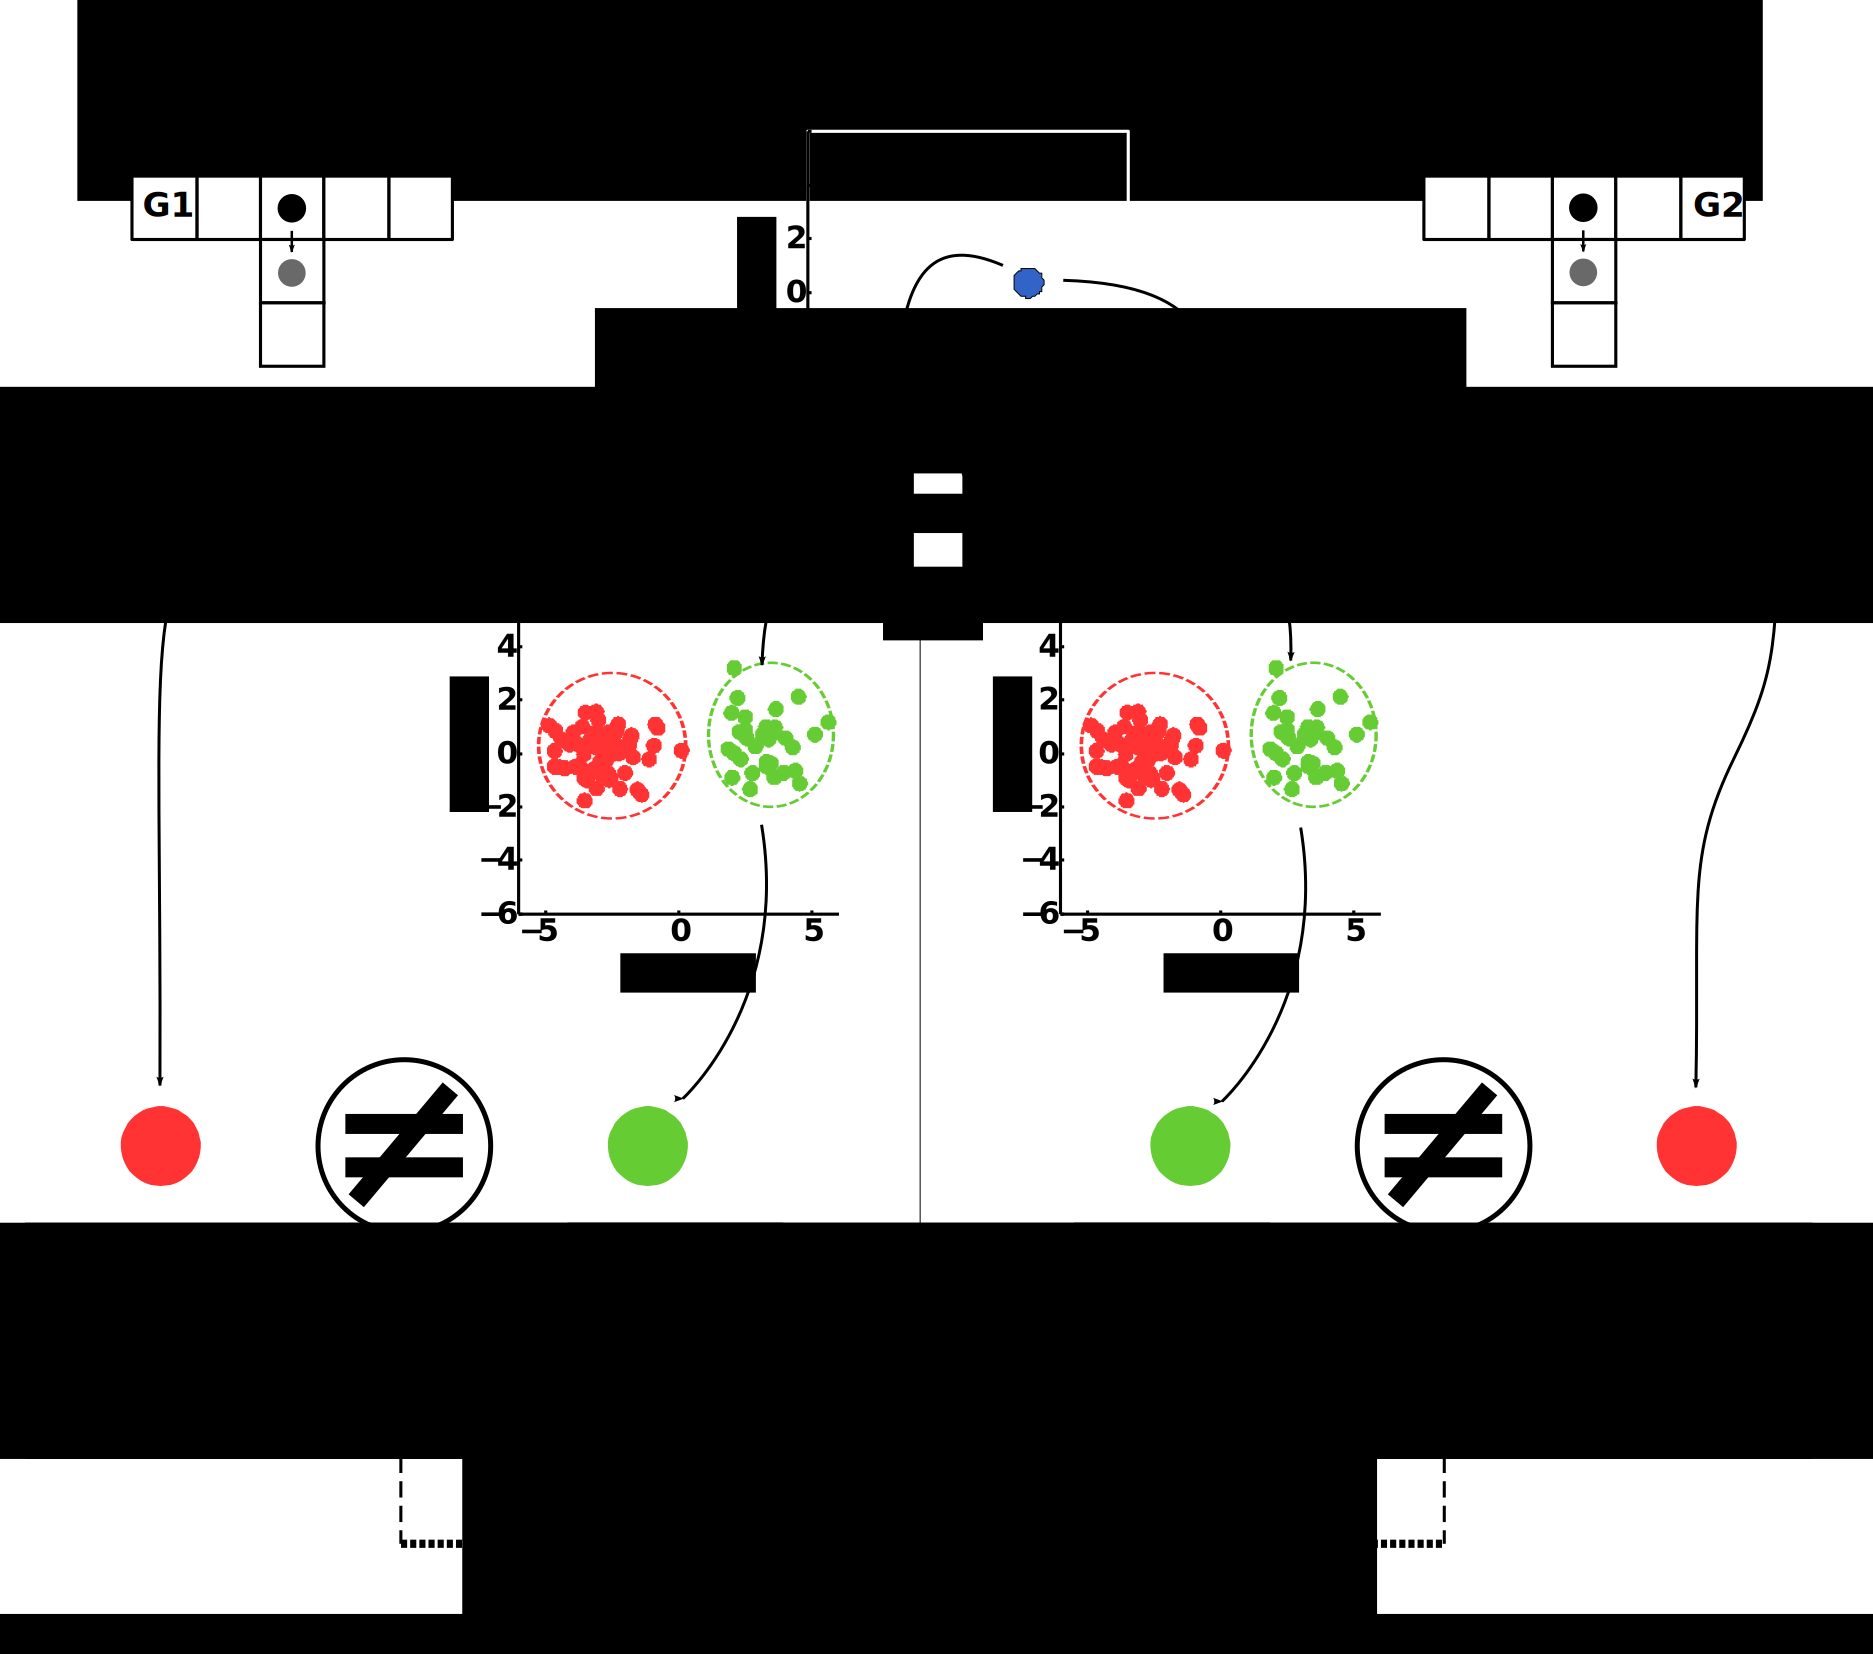
\includegraphics[width=\threeplanningwidth\columnwidth]{\visualspdf/planning/planning_up_down_expected_unmatched.pdf}
  \caption{Matching between expected labels and the prediction of a teaching signal sample on the right side of the feature space for the two hypothesis if the agent performs action down in state 3 and the two hypothesis currently have a symmetric interpretation of signals from Figure~\ref{fig:planningupdown}. Both hypothesis agree that the label associated to a signal on the right side of the feature space does not match with the label predicted given the frame and the state-action pair considered. Therefore there is no uncertainty associated to this state-action pair and the agent should not select action down in order to disambiguate between hypothesis.}
  \label{fig:uncertaintymeaningupdownexpectedright}
\end{figure}

This same process can be executed for any teaching signal. For example, as depicted in Figure~\ref{fig:uncertaintymeaningupdownexpectedleft}, considering a teaching signal on the left side of the feature space, if the agent performs action down in state 3, both hypothesis agree that this particular signal is expected. Hypothesis 1 expects a signal of meaning ``incorrect'', and the teacher signal is classified as being of class ``incorrect''. Hypothesis 2 expects a signal of meaning ``incorrect'' and the teacher signal is classified as being of class ``incorrect''. Therefore receiving this particular signal after taking action down in state 3 has low uncertainty.

\begin{figure}[!ht]
  \centering
  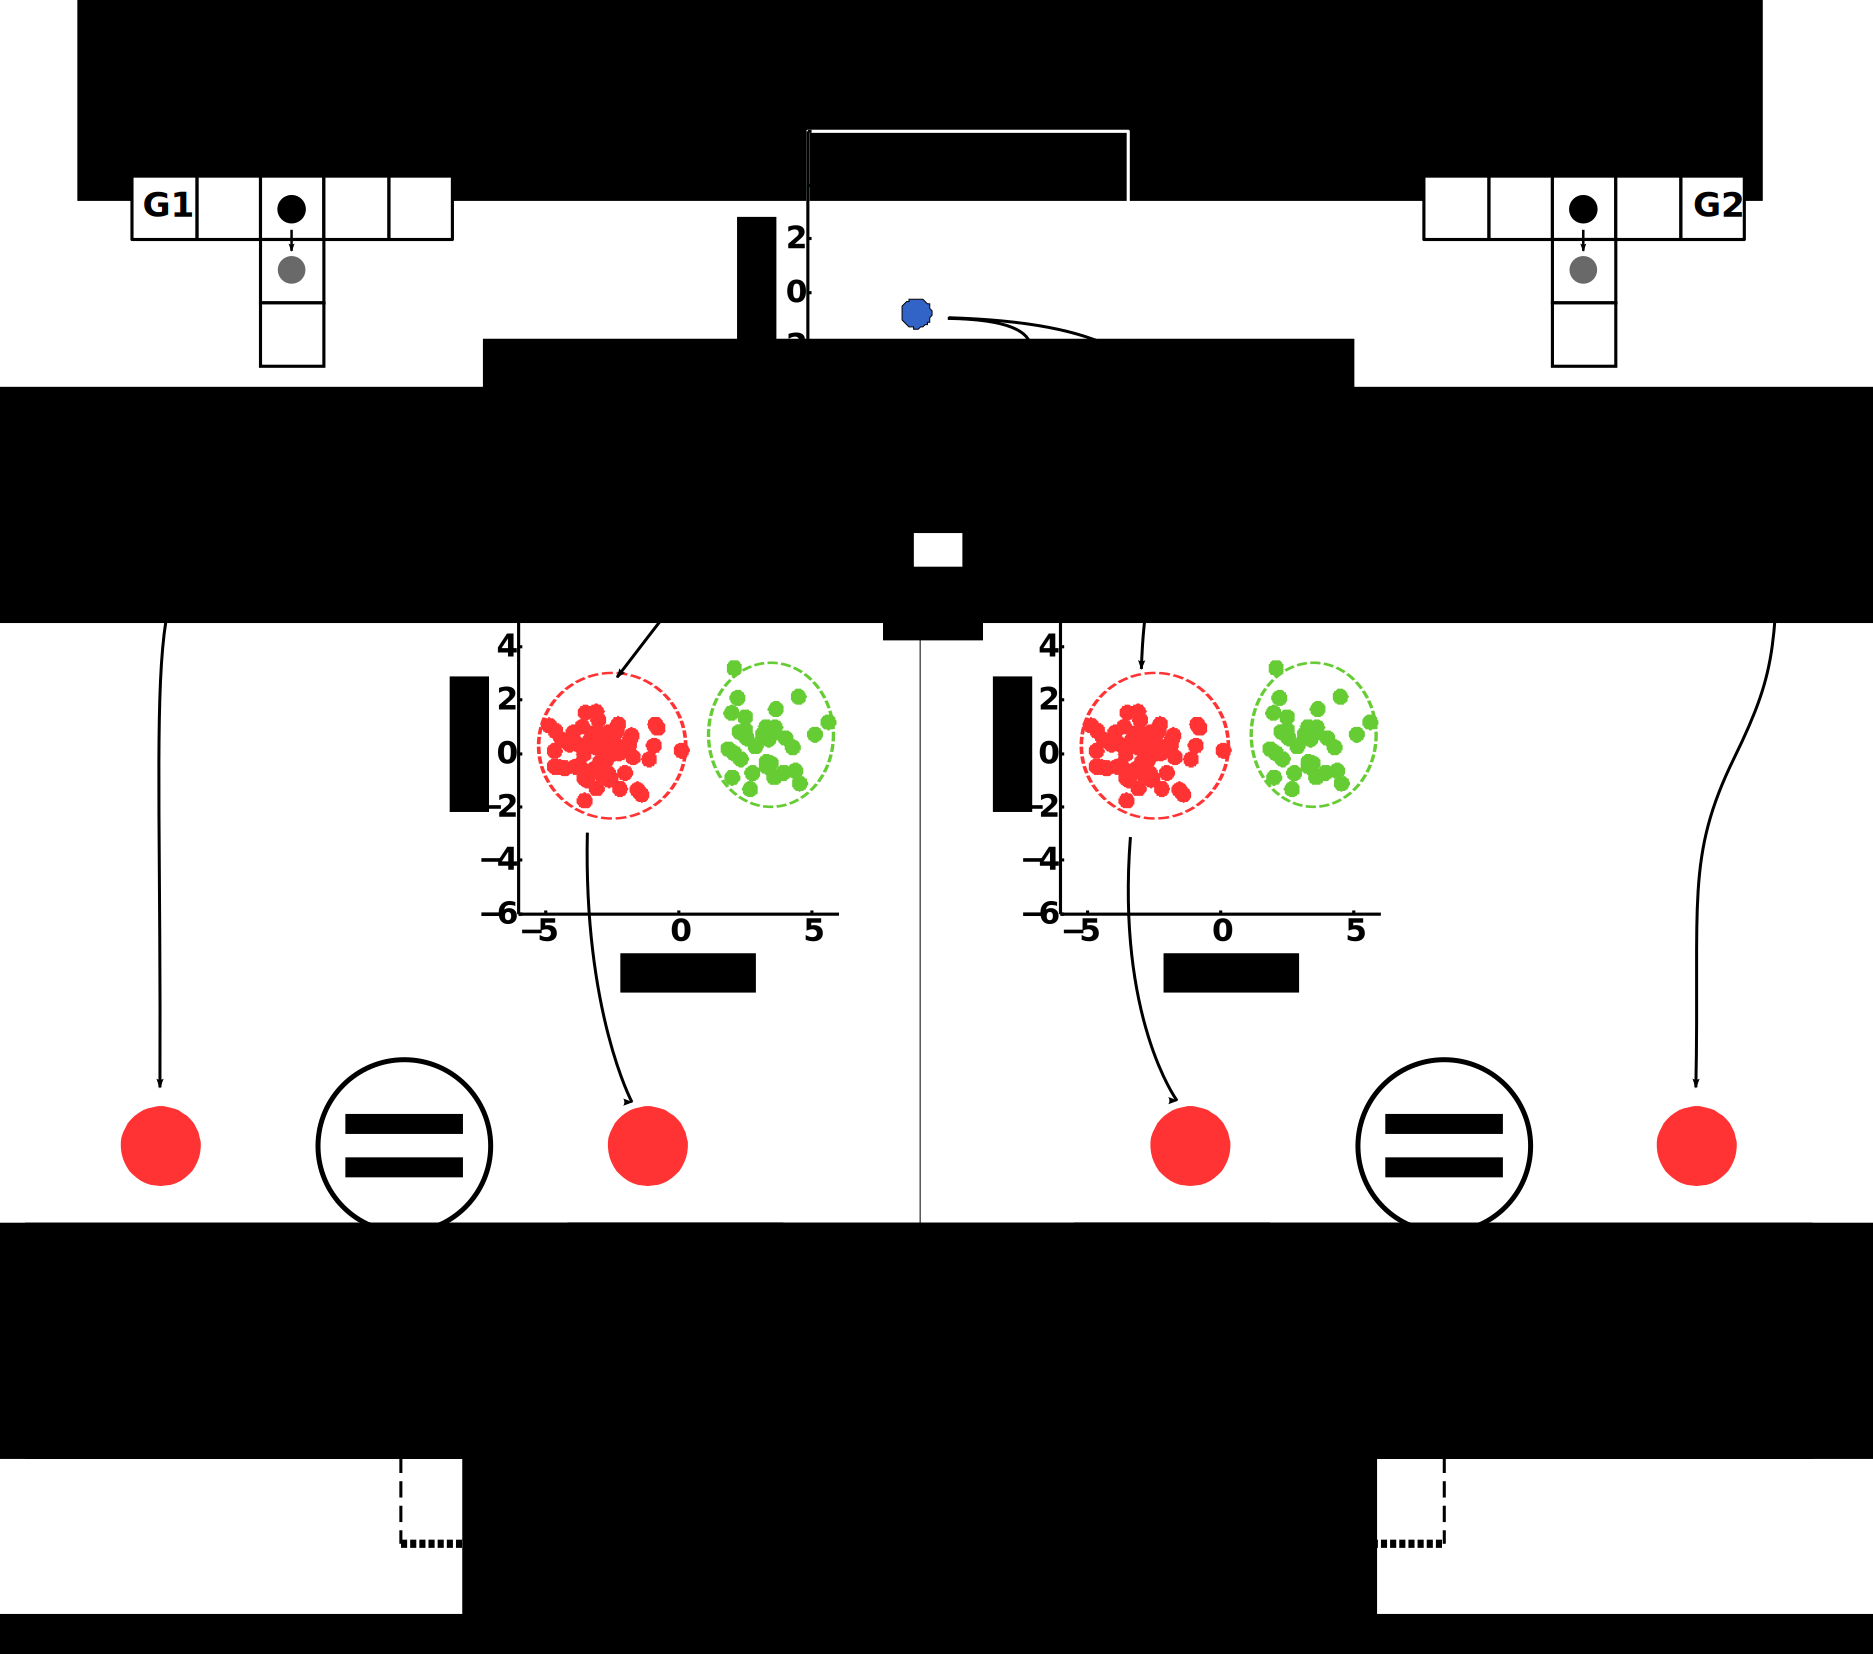
\includegraphics[width=\threeplanningwidth\columnwidth]{\visualspdf/planning/planning_up_down_expected_matched.pdf}
  \caption{Matching between expected labels and the prediction of a teaching signal sample on the left side of the feature space for the two hypothesis if the agent performs action down in state 3 and the two hypothesis currently have a symmetric interpretation of signals from Figure~\ref{fig:planningupdown}. Both hypothesis agree that the label associated to a signal on the left side of the feature space match with the label predicted given the frame and the state-action pair considered. Therefore there is no uncertainty associated to this state-action pair and the agent should not select action down in order to disambiguate between hypothesis.}
  \label{fig:uncertaintymeaningupdownexpectedleft}
\end{figure}

However for action left, the two hypothesis disagree on whether such signals are expected or not given the state-action pair considered. As depicted in Figure~\ref{fig:uncertaintymeaningupdownunexpectedright}, when selecting action left in state 3 and if the user sends a signal in the right part of the feature space, hypothesis 1 expects a signal of meaning ``correct'', and the teacher signal is classified as being of class ``correct''. And hypothesis 2 expects a signal of meaning ``incorrect'' and the teacher signal is classified as being of class ``correct''. Therefore receiving this particular signal after taking action down in state 3 is expected for hypothesis 1 but not expected for hypothesis 2, there is high uncertainty.

\begin{figure}[!ht]
  \centering
  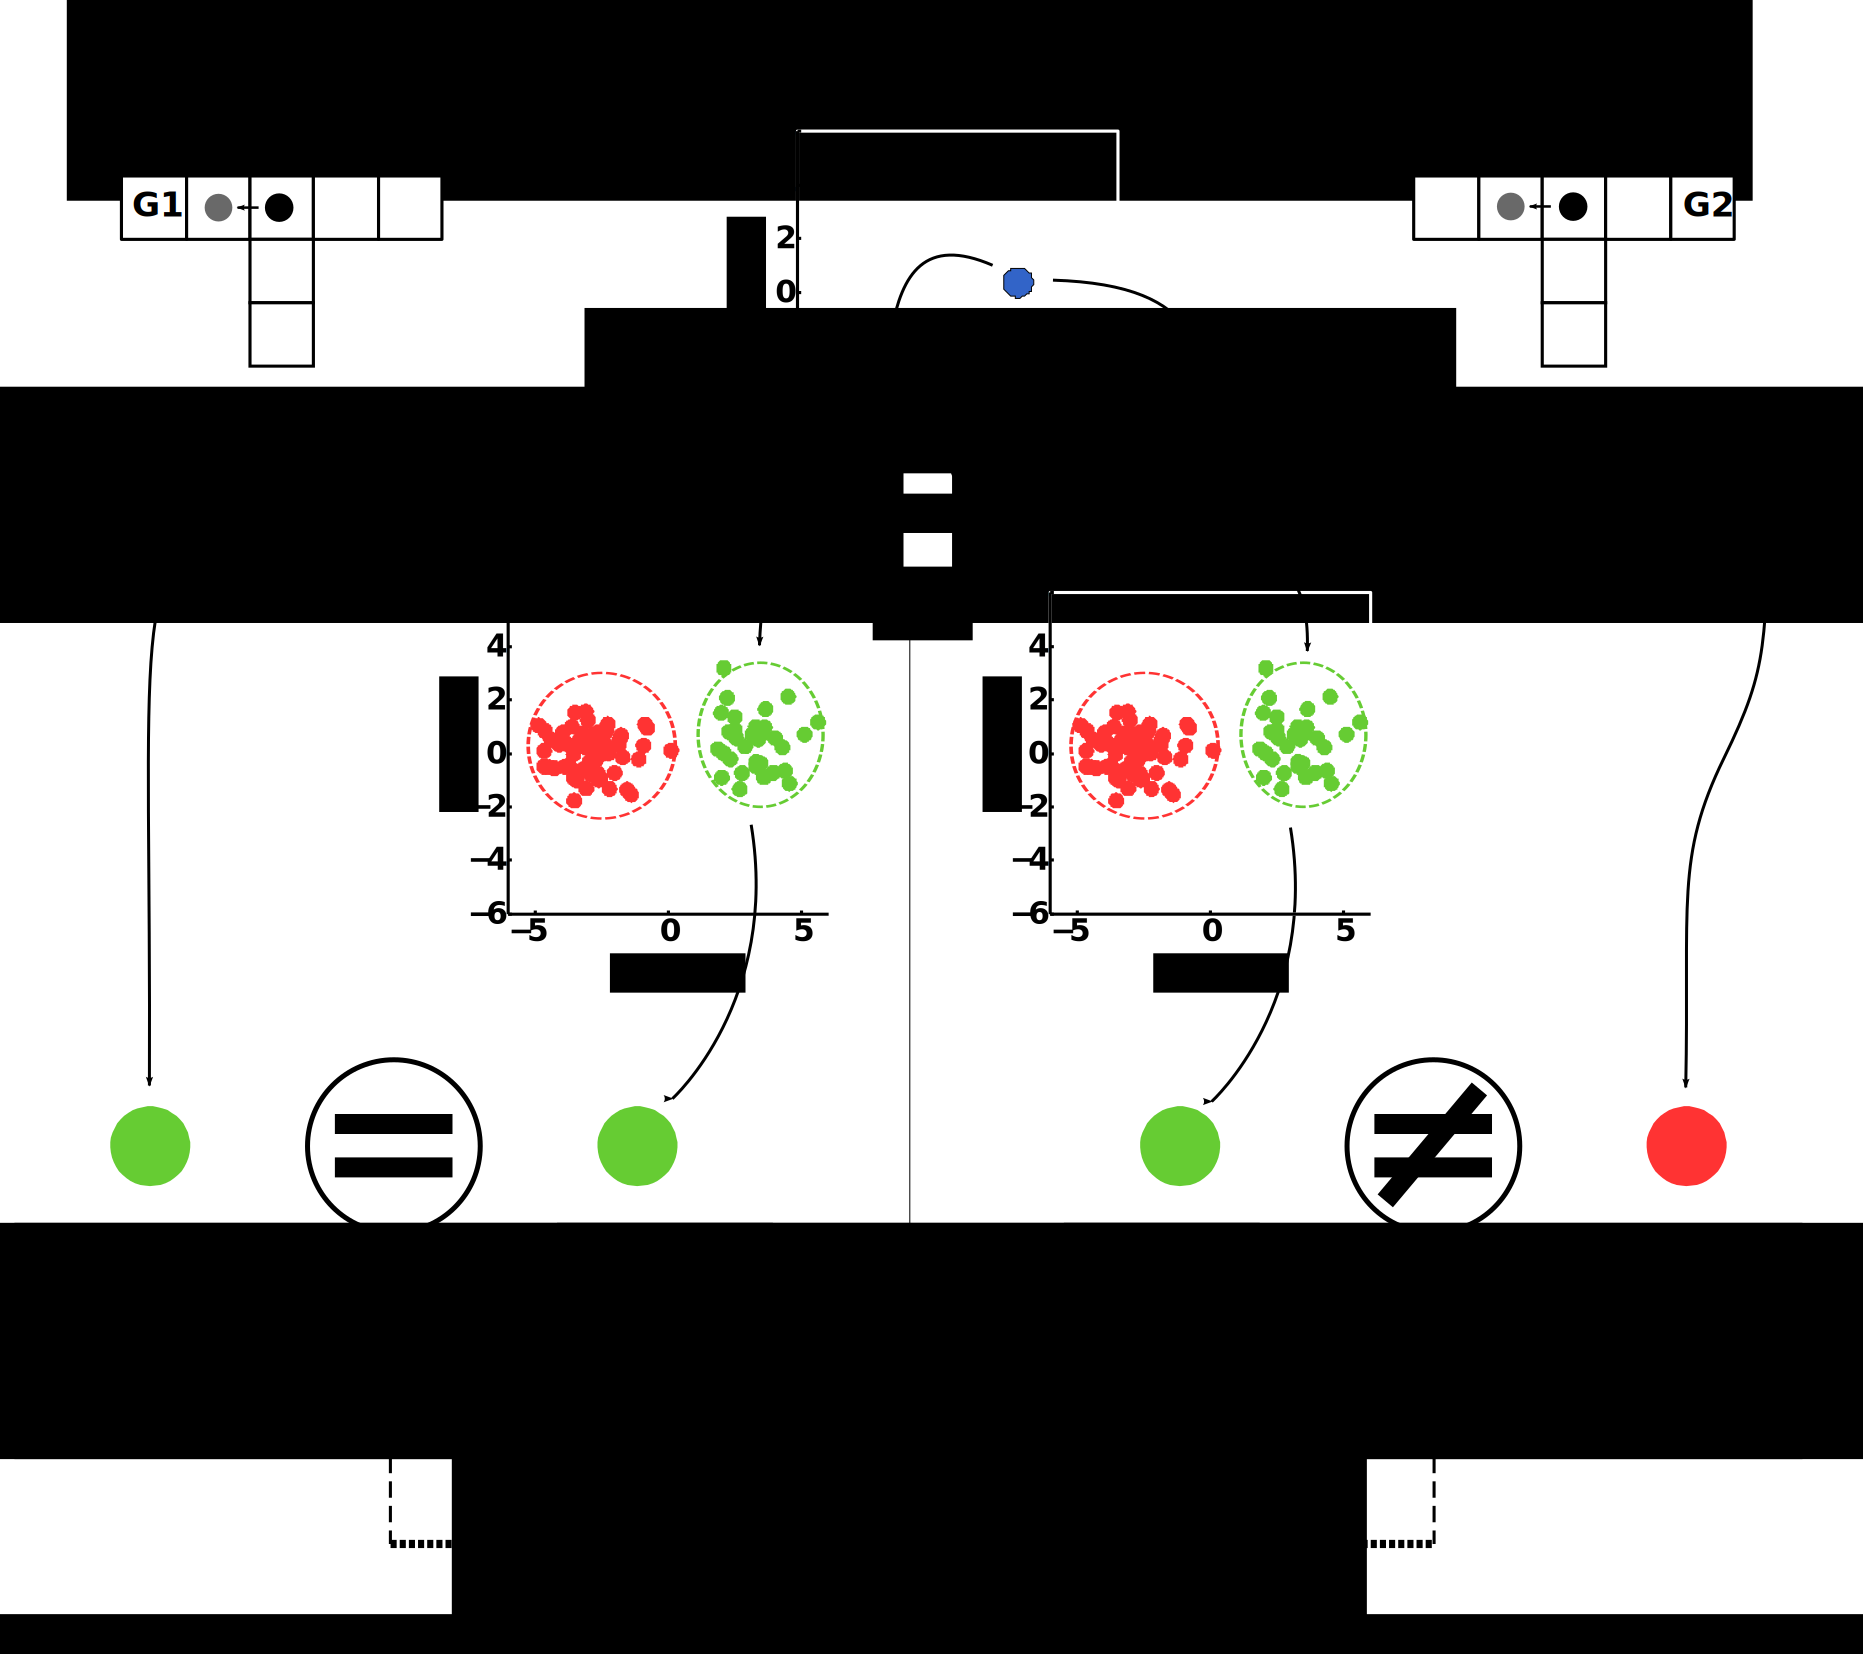
\includegraphics[width=\threeplanningwidth\columnwidth]{\visualspdf/planning/planning_up_down_unexpected_right_signal.pdf}
  \caption{Matching between expected labels and the prediction of a teaching signal sample on the right side of the feature space for the two hypothesis if the agent performs action left in state 3 and the two hypothesis currently have a symmetric interpretation of signals from Figure~\ref{fig:planningupdown}. Hypothesis 1 says a signal on the right side of the feature space means ``correct'' which was expected given the interaction frame, while hypothesis 2 expected a signal meaning ``incorrect'' but classify the signal as ``correct'' which was not expected. Therefore there is high uncertainty associated to this state-action pair and the agent should better perform action left in order to disambiguate between hypothesis.}
  \label{fig:uncertaintymeaningupdownunexpectedright}
\end{figure}

Similarly, as depicted in Figure~\ref{fig:uncertaintymeaningupdownunexpectedleft}, considering a teaching signal on the left side of the feature space, if the agent performs action left in state 3, hypothesis 1 expects a signal of meaning ``incorrect'', and the teacher signal is classified as being of class ``incorrect''. And hypothesis 2 expects a signal of meaning ``incorrect'' and the teacher signal is classified as being of class ``correct''. Therefore receiving this particular signal after taking action down in state 3 is not expected for hypothesis 1 but expected for hypothesis 2, there is high uncertainty.

\begin{figure}[!ht]
  \centering
  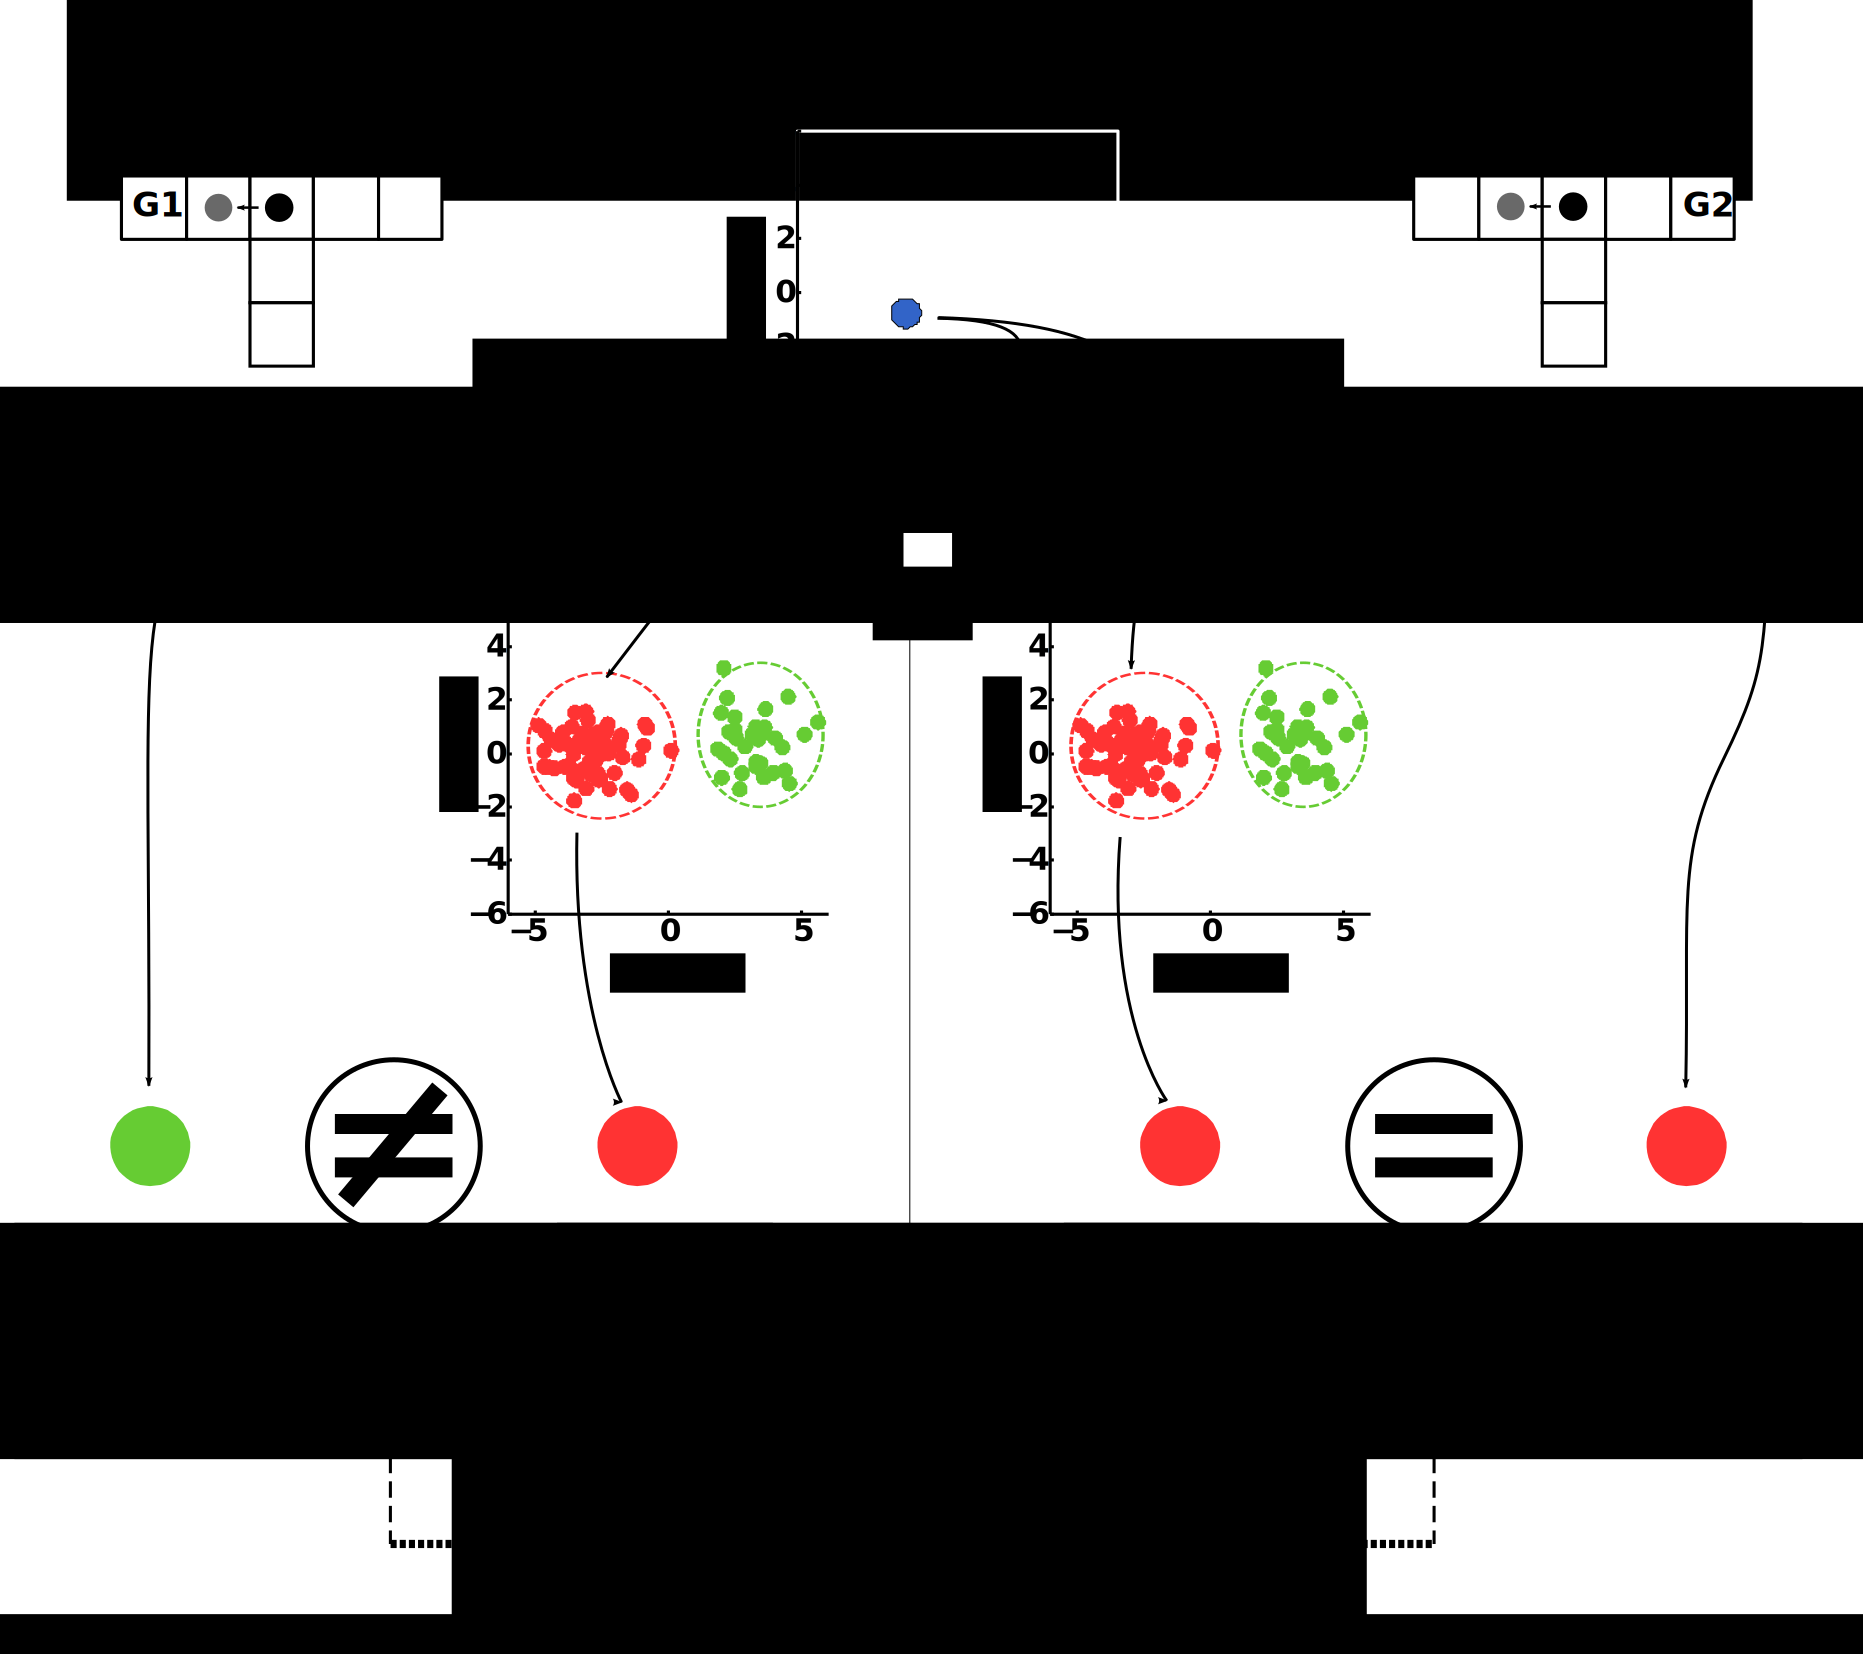
\includegraphics[width=\threeplanningwidth\columnwidth]{\visualspdf/planning/planning_up_down_unexpected_left_signal.pdf}
  \caption{Matching between expected labels and the prediction of a teaching signal sample on the left side of the feature space for the two hypothesis if the agent performs action left in state 3 and the two hypothesis currently have a symmetric interpretation of signals from Figure~\ref{fig:planningupdown}. Hypothesis 1 says a signal on the left side of the feature space means ``incorrect'' which was not expected given the interaction frame, while hypothesis 2 expected a signal meaning ``incorrect'' and classify the signal as ``incorrect'' which is what was expected. Therefore there is high uncertainty associated to this state-action pair and the agent should better perform action left in order to disambiguate between hypothesis.}
  \label{fig:uncertaintymeaningupdownunexpectedleft}
\end{figure}


%%%%%%%%%%%%%%%%%%%%%%%%%%%%%%%%%%%%%%%%%%%%%%
%%%%%%%%%%%%%%%%%%%%%%%%%%%%%%%%%%%%%%%%%%%%%%
%%%%%%%%%%%%%%%%%%%%%%%%%%%%%%%%%%%%%%%%%%%%%%
%%%%%%%%%%%%%%%%%%%%%%%%%%%%%%%%%%%%%%%%%%%%%%
%%%%%%%%%%%%%%%%%%%%%%%%%%%%%%%%%%%%%%%%%%%%%%
\section{Illustration of the gridworld scenario}
\label{appendix:gridworld}

In chapter~\ref{chapter:planning}, we consider a 5x5 grid world, where an agent can perform five different discrete actions: move up, down, left, right, or a ``no move'' action. The user goal is to teach the agent to reach one (unknown to the agent) of the 25 discrete positions which represent the set of possible tasks. We also consider the user is providing feedback on the agent action. We illustrate in Figure~\ref{fig:appendix:gridworldfeedback}, a smaller 3x3 grid world example and the results of the hypothetic labeling process. As the teacher is providing feedback with respect to hypothesis 1, the labeling process for hypothesis 1 is more coherent with the spacial organization of the data. We note that hypothesis 9 has symmetric properties with hypothesis 1 but the use of the ``no move'' allow to break that symmetry.

\begin{figure}[!ht]
  \centering
  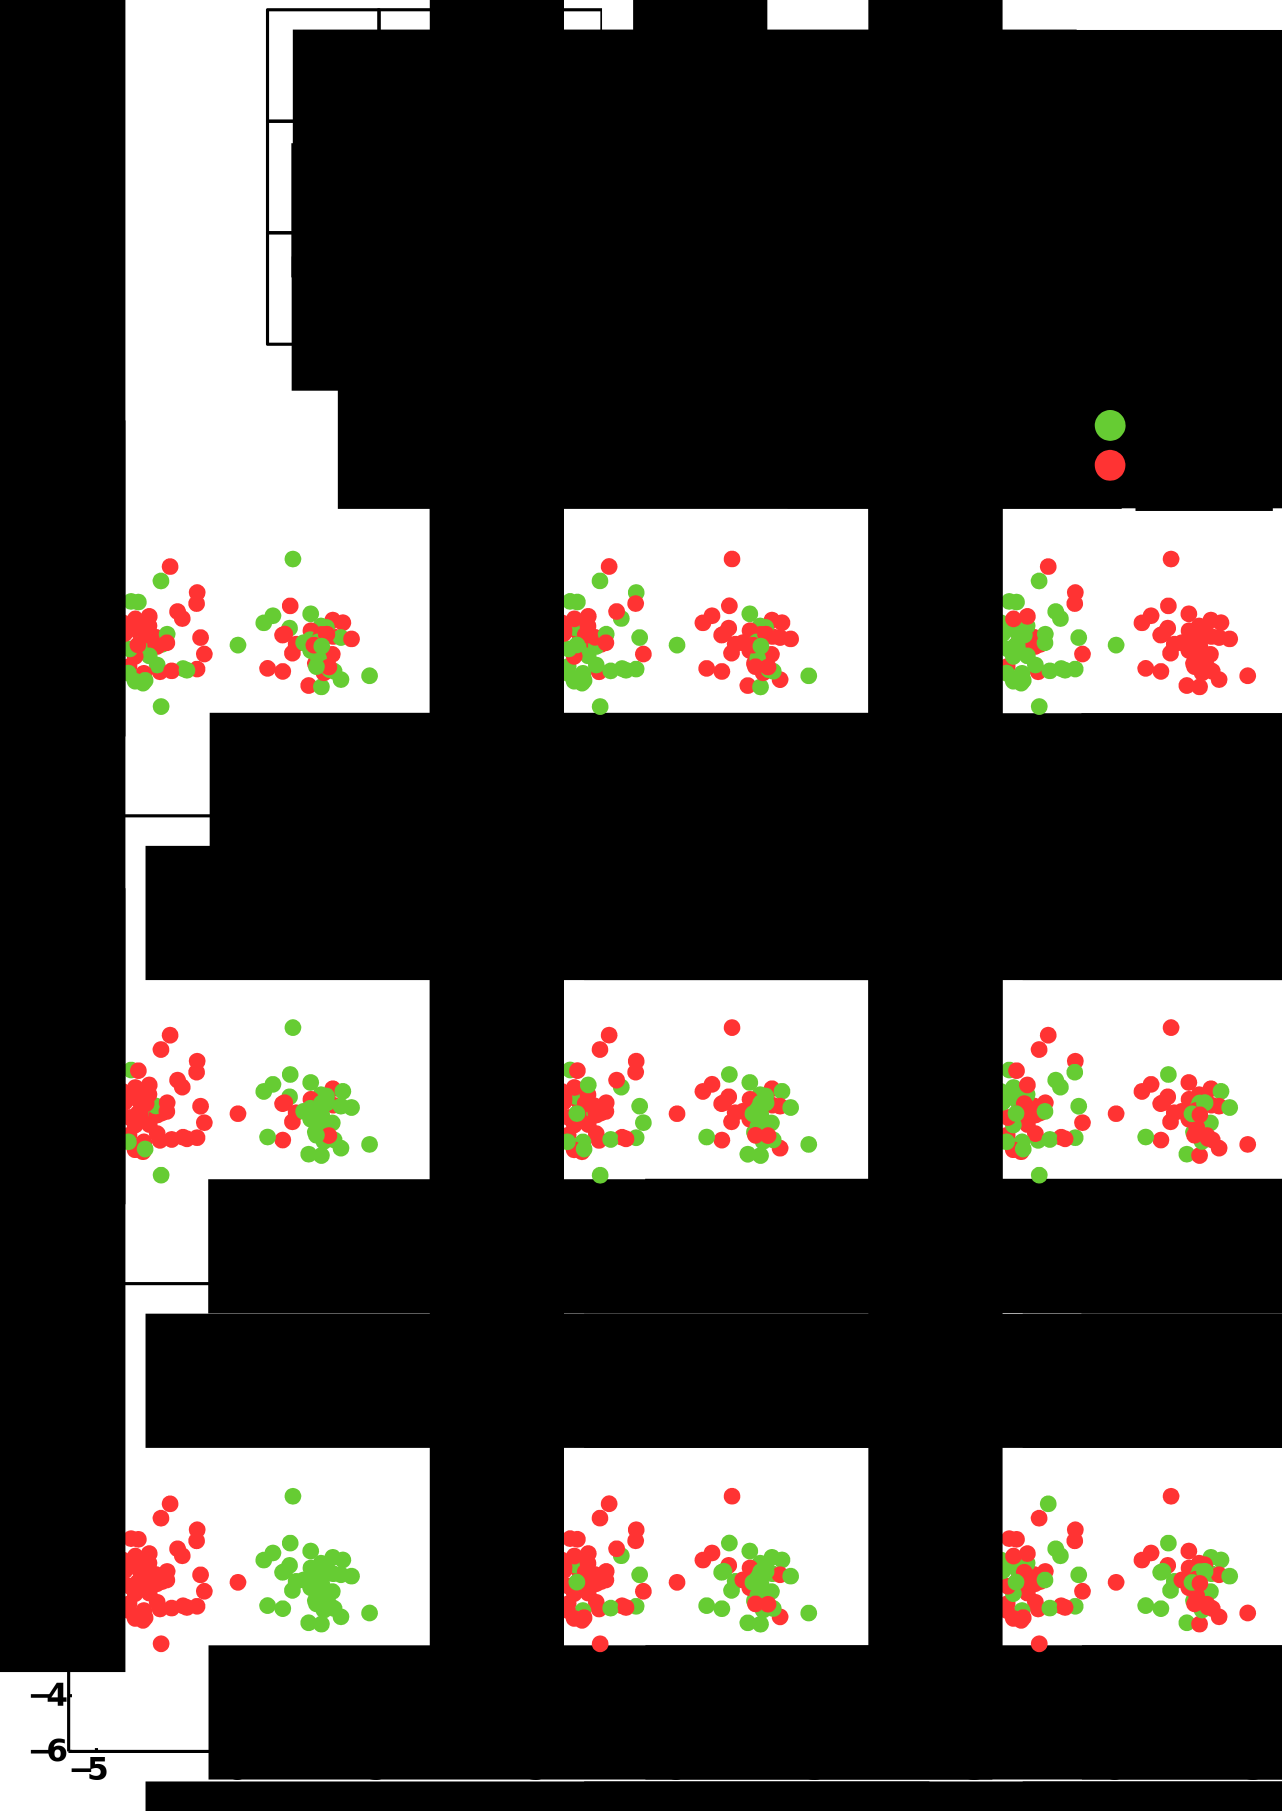
\includegraphics[width=\columnwidth]{\visualspdf/gridworld/gridworld_feedback.pdf}
  \caption{A schematic view of a 3x3 grid world scenario. There is nine possible hypothesis and the agent is acting randomly for this example. We show the results of the per hypothesis labeling process considering the feedback frame. The teacher is providing feedback with respect to hypothesis 1. The labeling process for hypothesis 1 is more coherent with the spacial organization of the data which indicates it is the one taught by the user. Hypothesis 9 has symmetric properties with hypothesis 1 but the use of the ``no move'' allow to break that symmetry.}
  \label{fig:appendix:gridworldfeedback}
\end{figure}








